\chapter{Data Acquisition}
\label{ch:sp-daq}

%%% todo

\fixme{\textbf{Authors:}

  See \url{https://wiki.dunescience.org/wiki/Technical_Design_Report}
  for general guidance. 

  While this chapter is still in outline, \textbf{check that it hits all
  the required points} some of which are:

  We are to describe a \textbf{baseline} or \textbf{process to
  decide a baseline}.

  \textbf{BE SUCCINCT} $TDR \approx IDR + 10\%$, goal is 50 pages for
  this chapter. 

  You are encouraged to produce \textbf{tech notes} with any
  supporting verbosity which may be referenced.

  State requirements and demonstrate how they are met, use
  standardized requirements table.

  Emphasize safety and professionalism (projectisms: cost, schedule,
  risks, interfaces).}

\metainfo{Some sections of this chapter must be written generically
  and without any reference to module-specific terms. They are marked
  with an orange ``fixme'' box. 
  Yellow info boxes like this one provide guidance for the content. 
  This guidance is not comprehensive so authors may provide additional
  information but retaining \textbf{conciseness} and \textbf{not
    repeating} info in other section is required.}

\section{Introduction}
\label{sec:fd-daq:introduction}
% \fixme{module-generic}

% \metainfo{A brief introduction to this chapter describing what will be
%   described.  This is \textbf{not} an overview of the DAQ itself.
%   Keep it brief. Do \textbf{not} write a conceptual overview here,
%   that is below, reference it. 
%   Do \textbf{not} use module-specific language but \textbf{do}
%   describe how commonalities are described in text shared by both
%   SP/DP volumes and specialized sections appear only in their
%   respective volume. 
%   \textbf{Do} describe the lexicographical convention used to demark
%   shared sections (this needs coordination with other chapters in the
%   same boat).}

The design of the \dword{dune} \dword{fd} \dfirst{daq} system is described in this chapter.  The DAQ services all \dword{fd} \dwords{detmodule}.  Most  aspects of the design are identical across the different \dwords{detmodule} and they are described in sections below which are reproduced verbatim in this \dword{daq} chapter in each \dword{detmodule} TDR volume.  A minority portion of the DAQ design that must be tailored to meet module-specific requirements are documented in sections below which are unique to each \dword{detmodule} TDR volume.  These sections are identified simply by their module-specific language.

The sections below begin with the requirements for and interfaces between DAQ and other DUNE systems.  A section comparing the \dword{protodune} experiment with DUNE is given to highlight important information learned from that prototype and what still must be understood.  The subsequent section describes the design itself.  The chapter finishes with giving details on project management issues such as production, installation, cost, schedule, safety, and other items.

\section{Requirements}
\label{sec:fd-daq:requirements}
\fixme{module-generic}

%\metainfo{One sentence introducing the contents of this section.}

The DUNE FD DAQ system must meet the requirements 
summarized in Table~\ref{tab:fd-daq:requirements}. The system is
designed to meet these requirements, and does so by following the key
specifications provided in the following subsection. Some of those
specifications are derived from the overall DUNE FD top level requirements.

\begin{dunetable}
[Requirements of the DUNE FD DAQ System.]
{cllcll}
{tab:fd-daq:requirements}
{The requirements of the DUNE FD DAQ System.}
Requirement ID & Name & Description & Value & Rationale & Validation \\ \toprowrule
1 & High-energy Trigger & The detector shall trigger on the visible
energy of underground physics events with $>$99\% efficiency. &
$>$\SI{100}{\MeV} & Study of these events is part of the DUNE mission.
Cosmic rays are also essential for calibration. & Refer to physics
TDR. \\ \colhline
2 & Low-energy Trigger & The detector shall be capable of triggering
on the visible energy of single low energy neutrino interactions with
$>$50\% efficiency. &
$>$\SI{10}{\MeV} & Study of these events enables supernova and solar
neutrino physics studies and provides monitoring of detector. & Refer
to physics TDR. This value is an achievable parameter; lower
thresholds may be possible. \\ \colhline
3 & Beam Trigger & The detector shall trigger on the visible energy of
beam interactions with efficiency high enough that it has a
sub-dominant impact on physics sensitivity. & $>$\SI{100}{\MeV} &
Study of these events is the primary DUNE mission. & Techniques for
doing this have been run succesfully in MINOS, NOvA and T2K. This value
is an achievable parameter; lower thresholds are possible. \\
\colhline
4 & Calibration Trigger & The detector shall provide triggers to and
trigger on calibration stimuli and tag the data from these triggers as
such. & & Calibration is essential to attain required detector
performance. & Refer to physics TDR. \\ \colhline
5 & SNB Trigger & A trigger shall be generated when a collection of
low-energy trigger candidates is detected that constitute a candidate
supernova burst. & $<$1\/month on average & Study of SNB is part of
the DUNE mision, this is one of the ways to collect such data. & Refer
to physics TDR. \\ \colhline
6 & Physics Event Records & The DAQ shall merge the data from one
physics trigger together in a data unit suitable for offline
analysis. Furthermore, tags shall be provided along with it to allow the data
collection conditions at the time and the livetime to be determined. &
& Allows the data conditions and the livetime at the time of the
record to be determined. & Required for offline physics analysis. \\ \colhline
7 & DAQ Deadtime & The DAQ shall operate without any deadtime between
acquisition of data for single neutrino interactions and
backgrounds. & 0\% & Zero deadtime makes physics analysis bookeeping
for overall livetime much simpler, and allows acquisition of neutrino
evens even with accidentals from backgrounds such as radiologicals. &
0\% is an achievable inter-event deadtime but a small deadtime would
 not significantly compromise physics sensitivity. \\ \colhline
8 & High-level Trigger & The DAQ architecture shall provide a parallel
processing farm once events have been built to enhance data selection
capability and leaverage the available bandwidth to permanent
storage. & & & \\ \colhline
12 & Readout Data Buffering & Each readout shall store
data continuously in a ring so that when a trigger condition is
satisfied, the data from earlier (covering the trigger decision
latency and some additional lookback) is possible. & $>$\SI{4}{s} & \\
101 & Supernova Deadtime Minimization & The DAQ system shall allow
data collection to continue in some parts of the detector when a fault
or crash interrupts data collecting in one part. & & & \\ \colhline
102 & Remote operation & The data collection shall be controllable
easilly from remote locations and the authentication shall be
implemented to allow exclusive control. & & & \\ \colhline
103 & Expert mobile notification\/status & & & Viewing the status and
receiving notifications on mobile devices shall be facilitated.  & & &
\\ \colhline
105 & Combined Operation & The SP-DAQ shall be integrated fully with
and operate consistently to the DP-DAQ and the near detector DAQ to
allow shifts of all to be taken from one location by a small number of
operators. & & & \\ \colhline
106 & Remote power and reset & Some form of slow control system & & &
\\ \colhline
111 & Partitioning & The DAQ system shall permit concurrent runing of
different subsets of the \dword{fd} elements in \dword{daqpart} to permit
detector development or specialised runs in parallel with standard
data taking. & & & \\ \colhline
112 & Data Flow Orchestrator & & & & \\ \colhline
113 & Configuration & & & & \\ 
\end{dunetable}

%\fixme{The following are notes that need integration.}
%  \item Front-end Buffer sub-system shall provide sufficient continuous storage of the full detector data flow to allow for the delay needed by the Data Selection subsystem to form a trigger decision, for the resulting trigger command to be executed by the back-end Egress sub-system and for the selected data to be received by the back-end.
%  \item The Buffer sub-system shall further provide sufficient continuous storage of the full detector data flow to allow selecting a subset prior to an SNB trigger decision for a period of time indicated by current SBN models. 
 % This pre-trigger time is taken to be $\approx$10s.

 % \item The DAQ shall minimize downtime for data acquisition and whenever possible continue nominal operations in parallel with any subset being taken offline or employed for any exceptional use.
%  \item Transitioning between \dwords{daqrun} shall require little to no downtime and shall require no downtime for \dwords{daqpart} unrelated to the transition.  
 
\subsection{Specifications}
\label{sec:sd-daq:specifications}
\fixme{single-phase module}

%\item A \dword{daqrun} is identified with a \dword{daqrunnum}.
 % \item The components of the DAQ shall be asynchronous and loosely coupled and in particular no global control of their state shall be centrally controlled.  Synchronization shall be performed dynamically and in a distributed fashion. 
 % \item The DAQ shall be robust against intentional and unexpected removal and addition of individual components. 
  %  Single points of failure should not exist and may only be allowed based on a cost/risk analysis.
  %\item Detector coverage and DAQ data selection criteria shall be recorded.  Coincident with intentional changes and upon discovery of unintentional changes the DAQ shall transition to a new \dword{daqrun}.
 % \item Unexpected failures in the operation of DAQ components should be automatically detected, reported, and handled so as to minimize system and human reaction time and to minimize reliance on human intervention.

The overall DUNE FD requirements which drive the key specifications of the
DAQ system, as well as additional key DAQ system specifications, are
listed in Table~\ref{tab:sec-daq:specifications}.

%\metainfo{Include rows of top-level requirements table (``Schmitz''
% table) here. 
%  Augment that with any additional requirements of our determining. 
 % Eg: accept data from detector electronics, perform reduction to
 % satisfy output rate limit, allow for cross-module triggering,
 % collect beam activity with XX\%, SNB requirements, noise level,
  %total thermal and space envelop, etc....}
%
% \metainfo{Include message passing requirements and domains.}

[Specifications for the DUNE FD DAQ System.]
{cllcll}
{tab:fd-daq:specifications}
{The DUNE FD DAQ specifications, derived by either the DAQ or the top
  level requirements of the DUNE FD.} 
Requirement ID & Name & Description & Value & Rationale & Validation \\ \toprowrule
%THE FOLLOWING ARE selected from top level requirements, Nov. 5 version of xls sheet
1 & Minimum Drift Field & The drift field in the TPC shall be greater
than \mindriftfield, with a goal of \mindriftfieldgoal. & $>$250 V\/cm
(goal 500 V\/cm) & This provides a specification for the maximum
readout integration time for the DAQ & \\ \colhline
2 & Front-end electronics noise & The FE electronics shall contribute
no more than \elecnoisefe of noise, with a goal of ALARA. This
requirement is on total system noise; it is expected that random noise
on the FE will dominate. & $<$ 1000 enc & This provides a
specification for the data reduction that can be achieved by the DAQ. & \\ \colhline
%3 & Light Yield & The light yield shall be sufficient for measuring
%event time (and total intensity) of events with visible energy above
%\SI{200}{MeV}.  Goal is to make possible a \num{10}\% energy
%measurement for events with a visible energy of \SI{10}{MeV}. & $>$
%0.5 pe\/MeV & & \\ \colhline
4 & Time Resolution & The time resolution shall be less than \timeres
in order to assign a unique event time. & $<$ 1 microsecond & This
determines the required timing resolution of the DAQ
timing distribution and synchronization system. & \\ \colhline
%5 & Liquid Argon Purity & The LAr purity shall remain lower than
%\larpurity (with a goal of < \larpuritygoal). This corresponds to e-
%lifetime of 3 (10) ms. & $<$ 100 ppt (goal 30 ppt) & & \\ \colhline
12 & HV power supply ripple contribution to system noise & Power
supply ripple shall be adequately attenuated to guarantee that its
contribution to the overall system electronics noise (at
\SI{50}{\hertz} and in the \SI{30}{\kilo\hertz} region) is negligible.
& $<$ 100 enc & This provides a
specification for the data reduction that can be achieved by the DAQ.  & \\ \colhline
%16 & Detector Live Time & The detector shall operate stably at least
%\livetime of the time in order to collect the required physics data. &
%$>$ 90\% & The DAQ should contribute to the detector
%downtime by more than 1\%. & \\ \colhline
19 & ADC Sampling Frequency & The ADC sampling frequency shall be set
so as to extract maximal information without unecessarily increasing
data rate. & 2 MHz & This determines the size of data associated with
each trigger record. & \\ \colhline
20 & ADC dynamic range & The ADC dynamic range shall be at least
\adcdynrange, with a goal of \num{4070}:\num{1}. & $>$3000:1 (goal
4070:1) & This determines the size of data associated with
each trigger record. & \\ \colhline
22 & Data Rate to Tape & The DAQ shall provide capability for
triggering on events of interest in order to limit the total bandwidth
for events stored on tape. & $<$30 PB/year & This determines the
overall data reduction factor to be provided by the DAQ. &  \\ \colhline
25 & Non-FE Noise Contributions & All non-FE noise contributions shall
be much lower than the targeted noise level for the collection wires.
& $\ll$ 500 enc & This provides a
specification for the data reduction that can be achieved by the DAQ. \\ \colhline
27 & Introduced Radioactivity & Introduced radioactivity shall be less
than that from 39Ar. & ALARA & This provides a
specification for the data reduction that can be achieved by the DAQ.
& \\ \colhline
%28 & Dead Channels & Detector components shall be sufficiently
%reliable so as to ensure that dead channels do not exceed
%\deadchannels over the lifetime of the experiment. & $<$ 1\% & & \\
%THE Following are selected from josh klein's edited version of
%oct. 26 daq requirements sheet from Giles
11 & Localization of trigger & The trigger system shall be capable of
recording the time and the aproximate APA location of each trigger for
use in data reduction & & & \\ \colhline
13 & Trigger decision latency & The trigger decision time for single
interactions shall be made and delivered back to the continuous
storage element within a time of 1s 99\% of the time and within 2s 100\%
of the time and ALARA. & $<$\SI{1}{s} & & \\ \colhline
14 & Trigger window & The data around a trigger will be collected in a
programmable time window that is configurable by trigger type.
Excepting the SNB trigger (where data are writren to a different
destination), this shall be programmable within a minimum time of 20us
and a maximum of 30ms. & $<$\SI{20}{ms} & 30ms is well over 3 drift
times in even the lowest fields and seems to be easy to implement.
Programmable by trigger type allows optimisation of bandwidth in
system. & ProtoDUNE trigger window \\ \colhline
15 & SNB trigger window & When a SNB trigger is activated, the data
from the pre-trigger buffer and then the further incoming data shall
be stored in a non-volatile solid-state-drive  & & Primary physics
mission & \\ \colhline
16 & SNB deadtime & When the unallocated space in the SNB
solid-state-drives runs out, the SNB trigger shall not
overwriteexisting data in the solid-state-drives. & & The deallocation
of SSD space should be done rapidly, and is better than a policy of
overwriting by default. & \\ \colhline
17 & Livetime of triggers & A software programmable trigger priority
scheme shall be provided, this shall be implemented in a way that the
main physics triggers are never or rarely inhibited to enable the
live-time of these triggers to be easilly determined. & & For example,
to hold off calibration when the beam is expected, or to stop certain
triggers (e.g. calibration) during an SNB trigger.  Also to prioritize
an atmospheric neutrino trigger above a solar-neutrino trigger & \\
\colhline
21 & Trigger primitives from APAs & A real-time algorith shall
generate trigger primitives by search for "hits" on collection
wires. Trigger Primitves will include information that is at least the
channel number, the hit time, the pulse height or integral, and pulse
width. Trigger Primitive generation will have a latency that is small
enough that it can keep up with the detector data rate. & & & \\
\colhline
22 & Trigger candidates from APAs & A real-time algorithm shall search
for trigger candidates in each APA based on clustering of hit
collection wires, total event charge, and pulse widths. "Low-energy"
candidates will be identified for use in a supernova burst
trigger. The latency from the processing time shall be small enough
that candidate generation keeps up with data rate. & & & \\ \colhline
23 & Trigger Primitives from PDs & A real-time algorothm shall provide
trigger primitives by searching for "hits" in photon detectors and
provide. Trigger primitives will include at least channel number, hit
time and pulse height information. The latency shall be small enough
that it can keep up with detector data rate. & & & \\ \colhline
31 & Collection trigger primitives & The APA readout is currently only
required to generate trigger primitives from the collection planes,
and only on the wires facing the active detector. & & & \\
32 & Data compression & The APA readout may be losslessly compressed,
but no general lossy compression should be applied.   The compression
factor shall be at least 2. & 2 & & \\ \colhline
33 & Dead channels & Channels may be flagged by an operator as dead
and the DAQ shall disregard them in the trigger & & & \\ \colhline
34 & Noisy channels & Channels may be flagged by an operator as noisy
and the DAQ may disregard them in the trigger and apply a filtering
before compression to improve compresibility of these channels & & We
require that the compression algorithm does not inflate the data when
averaged over times of 10s of milliseconds, to avoid needing to build
in complex buffer management downstream for edge cases.  This
technique enables that simplification. & Examples of filtering that
could be applied to especially noisy channels would be to zero out the
low-significant-bits of the noisy channel, or to add adjacent channels
together to downsample to 1MHz. \\
\end{dunetable}

\subsection{Design Philosophy}

%\metainfo{Describe how the design addresses the requirements.}
The DUNE FD DAQ is designed to address the requirements listed in
\ref{sec:fd-daq:requirements}. The design itself facilitates a
reconfigurable and partitionable DAQ system, with great flexibility in how
the DAQ functionality is implemented in the system. 

Key philosophies are reflected in the design, in that the Readout System is
designed with the capability to receiving and buffer the entire raw data generated by
the full 10-kton module TPC and PDS systems for sufficient time to
facilitate O(1s)-delayed triggers. The Data Selection system
is capable of processing the raw data meeting data quality and noise
requirements in real time with negligible dead time, and provides
efficient triggering for the beam and non-beam physics program of
DUNE. The adopted DAQ partitioning scheme embodies a highly configurable detector and ensures
maximization of live time of the experiment. 
%Add about The Control,
%Configuration and Monitoring design ...

The system is furthermore designed to be reconfigurable and flexible
enough so as to facilitate future design evolution and optimization,
for example upgrades in FPGA and CPU data processing resources without changes to the
overall data flow architecture.

\subsection{Parameters}
\label{sec:sp-daq:parameters}
\fixme{single-phase module}

Table~\ref{tab:sp-daq:parameters} summarizes all important parameters
driving the DAQ design.

%\metainfo{Include a table which lists all important parameters driving
%  the design.  Sampling rate and resolution, channel count}


\section{Interfaces}
\label{sec:sp-daq:interfaces}
The DUNE FD DAQ system interfaces with the TPC Cold Electronics, PDS
Readout, Computing, CISC, and Calibration systems of the DUNE
FD, as well as with Facilities and Underground Installation. The
interfaces have been specified in the form of interface agreements,
and are summarized in Table \ref{tab:sp-daq:interfaces}. The system
interfaces are described in the following subsections. Interfaces with
Facilities and Underground Installation are described in Section~\ref{sec:sp-daq:production}.

\metainfo{Include interface summary and table here.}

\subsection{TPC Cold Electronics}
The DAQ and TPC Cold Electronics interface is specified in \cite{docid-6742}.
\metainfo{Data reception physical and logical, configuration information delivery.}
\subsection{PDS Readout}
The DAQ and PDS Readout interface is specified in \cite{docid-6727}.
\metainfo{Data reception physical and logical, configuration information delivery.}
\subsection{Computing}
The DAQ and Computing interface is specified in \cite{docid-7123}.
\metainfo{Buffer disk.  Agreement on sysadmin support and computer procurement, ssh gateways, non data networks.  Address reference how the data model described above is acceptable.}
\subsection{CISC}
\label{sec:sp-daq:interfaces-cisc}
The DAQ and CISC interface is specified in \cite{docid-6790}.
\subsection{Calibration}
The DAQ and Calibration interface is specified in \cite{docid-7069}.
\subsection{Timing System}
Because the Timing System of the DUNE Far Detector interfaces with
almost all detector systems and has a uniform interface to each of
them, rather than comprising a set of 
bilateral interface documents, a single interface document
\cite{docid-11224} describes all timing interfaces. 

\section{ProtoDUNE and DUNE Comparison}

\metainfo{Here we write what similarities and differences there are between ProtoDUNE and DUNE DAQ designs.}

\fixme{Notes:}
ProtoDUNE-SP/DUNE differences from Kurt's DFO and EB doc.
\begin{itemize}
\item Motivation: need to accommodate changes in the overall system and provide greater flexibility and granularity.
\item DUNE: input to DFO is the trigger command and provides all space/time addressing required to identify which data to collect.  Also includes is information about the trigger decision itself but the DFO merely passes this through to output.  The addressing contains all info needed for the DFO to act.
\item DUNE: The EB updates DFO as to what resources (buffers) it has available
\end{itemize}

\subsection{Detector Readout Hardware}

\metainfo{Compare and contrast design elements related to the detector readout hardware.}

\subsubsection{RCE}

\subsubsection{FELIX}

\subsection{Backend Event Building}

\subsection{Other}

\section{DAQ Design}
\label{sec:fd-daq:design}
% \fixme{module-generic}

% \metainfo{One sentence to introduce the section. 
%   Listing the subsections and describing which are generic and which
%   are X-phase specific.}

This section describes the DAQ design. 
It begins with a conceptual overview followed by sections giving the design of the DAQ subsystems. 
First come the \dword{ipc} and \dword{ccm} subsystems.
Next is the \dword{fe} data receiver and data handling and processing subsystems.
Then, the subsystems for data selection and the DAQ back-end are described Finally, the timing subsystem is presented and this section finishes with plans for design validation and development.


The following descriptions of the design are kept brief due to page limitations. 
More details are provided as technical notes as listed in Table~\ref{tab:fd-daq:tech-notes}.

\begin{dunetable}{|p{0.7\textwidth}|p{0.2\textwidth}|}{tab:fd-daq:tech-notes}{Summary of relevant and detailed DAQ technical notes.}
  Title & References \\
  DUNE Far Detector Data Volumes & \citedocdb{9240}\\
  The DAQ for the single phase DUNE Prototype at CERN & \citedocdb{8708}\\
  A System for Communication Between DAQ Elements & \citedocdb{10482}\\
  Data Selection for DUNE Beam and Atmospheric Events & \citedocdb{11215}\\
  Data orchestrator and event building for DUNE FD DAQ & t.b.d. \\
  DUNE Run Control, Configuration \& Monitoring (CCM) & t.b.d. \\
  DUNE DAQ Readout & t.b.d. \\
\end{dunetable}



\subsection{Overview}
\label{sec:fd-daq:design-overview}
%\fixme{module-generic}

\begin{dunefigure}{fig:daq-conceptual-overview}{DAQ Conceptual
    Subsystem Overview.  See text for description.}
  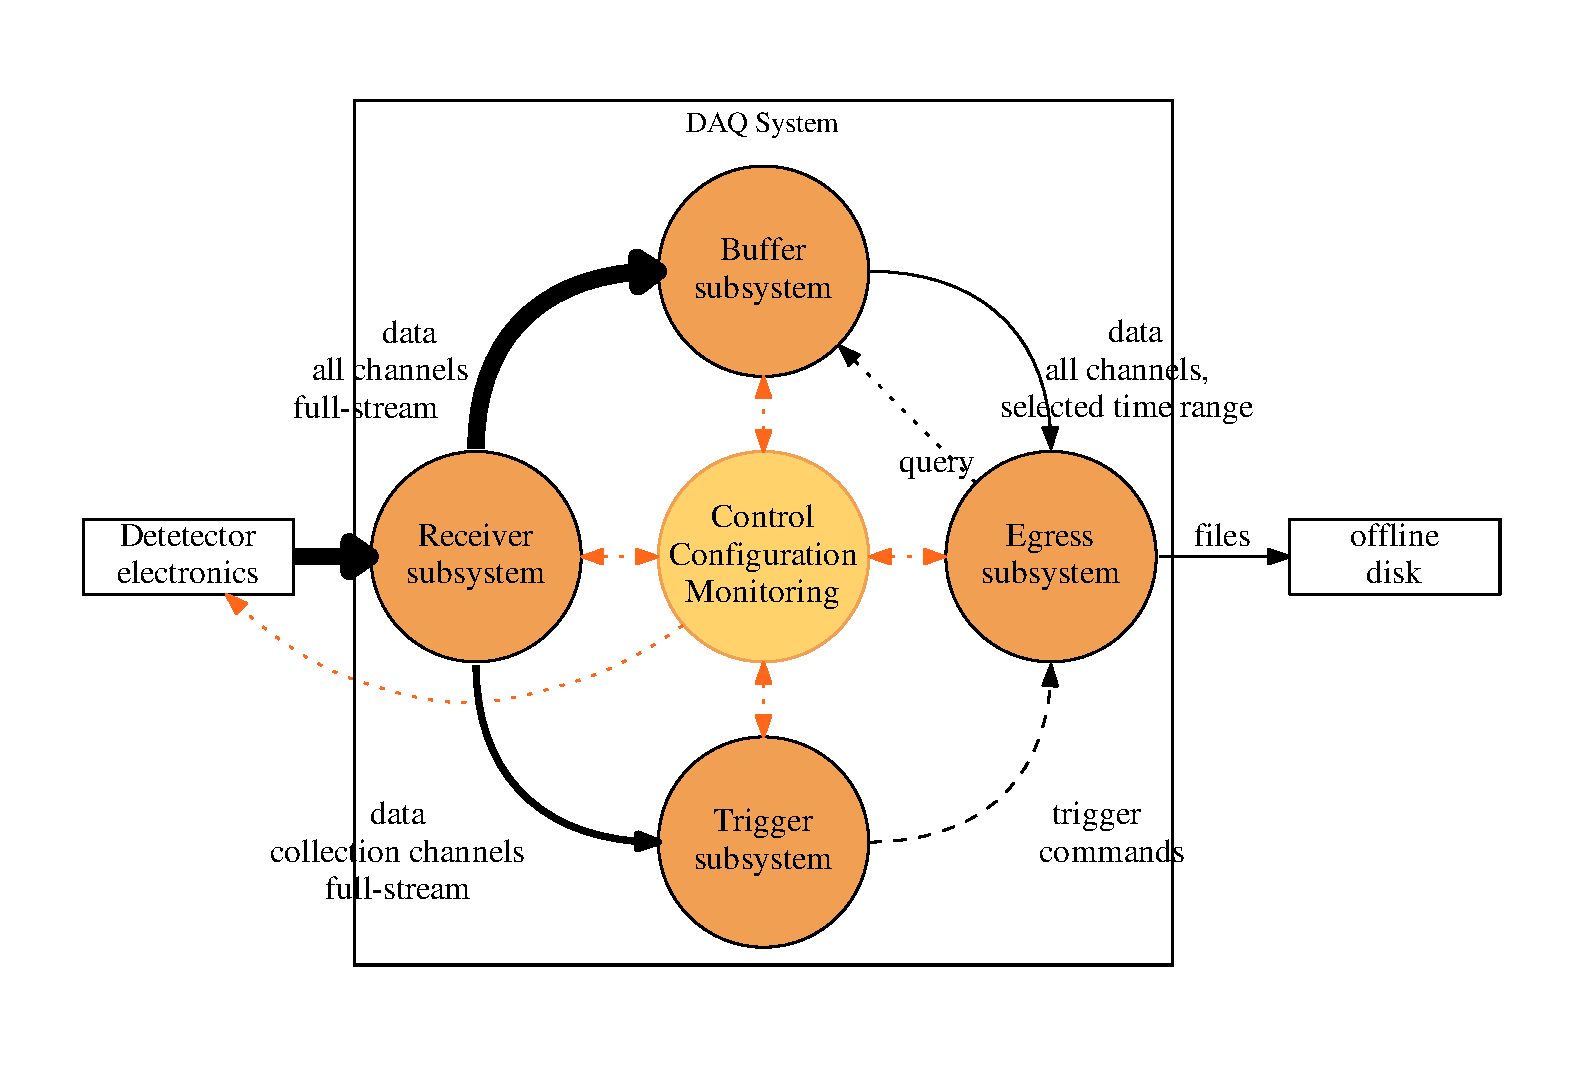
\includegraphics[width=0.8\textwidth]{daq-toplevel-conceptual.pdf}
\end{dunefigure}

% \metainfo{This is the \textbf{only} place to describe the conceptual
%   overview. 
%   Do \textbf{not} repeat this info in sections below. 
%   \textbf{Do} use \textbf{module-neutral} terms.
%   \textbf{Do} describe major interface between each subsystem (the edges between the circles in Fig~\ref{fig:daq-conceptual-overview}).
%   \textbf{Do} mention that concrete systems span portions of the
%   conceptual subsystems and how the following subsections are defined
%   along these concrete deliverable lines.}

An illustration of the conceptual parts which make up the DUNE FD DAQ is given in Fig.~\ref{fig:daq-conceptual-overview}. 
It applies to all \dword{fd} modules. 
The box in the illustration indicates the overall scope of the DAQ.
Each of the various concrete hardware and software subsystems describe later in this section provide a portion of one or more of the conceptual subsystems represented by the circles in the figure.
Approximately following the data flow through the DAQ, the concept starts with receiving input via optical fibers from the detector electronics (see Section~\ref{sec:fd-daq:design-felix}). 
The flow then bifurcates. 
The entirety of the input flow is buffered for a period of time sufficient to satisfy triggering and readout requirements (see Section~\ref{sec:sp-daq:design-fe-processing}). 
The second flow need contain only data that is to be used to form a \dword{trigdecision} (see Section~\ref{sec:sp-daq:design-selection-algs}).
The information in that decision is used by the egress subsystem to query back to the appropriate buffers and thus retrieve selected data (see Section~\ref{sec:fd-daq:design-backend}).
The results are aggregated and saved to files on nonvolatile storage media at which point custody is transferred to offline responsibility.
This is all orchestrated by the \dword{ccm} subsystem (Section~\ref{sec:fd-daq:design-run-control}) shown in the center of the figure.   The various information flows, represented by the arrows of the figure, ride on the \dword{ipc} subsystems (Section~\ref{sec:fd-daq:design-messages}). 

\metainfo{Include components summary and table here.  Need guidance on what is wanted.}

\fixme{Where will we describe partitions?}
As described more in Section~\ref{sec:fd-daq:partitions}, this conceptual picture is implemented in terms of a number of \dwords{daqpart} or instances. 
The primary set of partitions will exist underground in the \dword{cuc} in order to service the \dword{fd} modules. 
As described more in Section~\ref{sec:sp-daq:production} the DAQ will connect to and begin servicing portions of a \dword{fd} module after they are installed and commissioned. 
There will also be a DAQ presence in the \dword{itf} to support the work there during detector construction.
% \metainfo{Include physical location description}




\metainfo{For the remaining design sections: do not include directly validation info but rather place this information in section~\ref{sec:sp-daq:design-validation} and make references.}
  



\subsection{Inter-process Communication}
\label{sec:fd-daq:design-messages}
\fixme{module-generic}
\fixme{This can maybe moved toward the end of the section.}

The DAQ must transfer data between elements inside the DAQ and with external sources. 
This data is characterized by a variety of schema, latency and throughput. 
The system which provides for such transfers is generally termed \dfirst{ipc}.
For the most part, any \dword{ipc} system shall be reliable in that once a unit of data is sent it is successfully received as long as the recipient is accessible on the network and is operational. 
IPC systems should be robust against temporary interruption of network connectivity. 
A related and required function, described in Section~\ref{sec:fd-daq:design-run-control}, is that of \dword{daqdispre}. 
An IPC system may provide that functionality.

IPC, by construction, represents a system with a high degree of interconnection and associated complexity. 
It is recognized that implementations for different DAQ subsystems may provide their own native IPC solutions. 
The DAQ design shall support multiple such IPC \textit{domains} where they may be required to satisfy special requirements or if they are part of an existing sub-system solution. 
The number of domain IPC systems shall otherwise be minimized and where selected shall have well defined and non-overlapping scopes of usage. 
One IPC which is here termed the \textit{lingua franca} IPC, shall be selected after identifying options and evaluating them in terms of their performance, documentation, development simplicity and expectation of long term, open source and broad community support. 
The \textit{lingua franca} IPC system will form the basis of any new sub-system development which otherwise lacks an \textit{domain} IPC system and for connecting domain IPC systems via translating proxies.

An example of a subsystem that may support the \textit{lingua franca} IPC is the hierarchical trigger processing system provided by the data selection (Section~\ref{sec:sp-daq:design-selection-algs}. 
An a domain IPC is that which is employed by artDAQ which may provide the heart of the egress subsystem as described in Section~\ref{sec:fd-daq:design-backend}.
The DAQ shall also interface with external domains. 
For example, a two-way exchange of information shall exist between DAQ and \dword{cisc} as described in Section~\ref{sec:sp-daq:interfaces-cisc}.  

The protocols of the \textit{lingua franca} IPC shall be developed in conjunction with the DAQ sub-systems that use it. 
Across all usage, some commonalities are required. 
Every message shall carry a prefix of a fixed schema which shall include the following fields

\begin{itemize}
\item Identity of the dialect or version of \textit{lingua franca} IPC.  Mixing of dialects in one operation should not be performed.
\item Identifier of the protocol within the IPC.
\item Message type identifier.
\item A \textit{data time}.
\item Payload data following a message-type specific schema.
\end{itemize}

The \textit{data time} shall stamp the time of data acquisition of the data found in the message payload. 
As new output IPC messages are derived input the \textit{data time} shall be forwarded.
See Section~\ref{sec:daq:design:ccm:control} for how this timestamp is used to enact zero-downtime reconfiguration.


\fixme{Shall we name ZeroMQ specifically as the basis for the \textit{lingua franca} IPC?}

% \metainfo{Describe the domains requiring message passing.  A domain means parts that shall share the same message passing infrastructure.  Eg, the hierarchical trigger system is one.  The transfer of data between artDAQ nodes is another.  Run control, monitoring and logging is a third.  Some MP domains will exist in other consortia and must interface with DAQ MP domains.  Each internal or external interface must be at least listed.   Describe how effort will be conserved by minimizing the number of distinct domains to the extent it makes sense.  Some examples: two-way comms with CISC (CISC tells DAQ of HV it shut down, DAQ tells CISC about hardware health, DAQ process health, statistics on things like per-unit trigger rates), handling laser triggers (eg, want laser to only fire in between beam spills).}

% \metainfo{We may not be ready to give concrete designs for every domain.  Where this is the case, we must describe a plan for determining the IPC system for each domain.}

%\metainfo{IPC must support redundant paths for trigger information, especially at the MLT level and above, to assure robustness.}


\subsection{Control, Configuration and Monitoring}
\label{sec:fd-daq:design-run-control}
\fixme{module-generic}

\metainfo{Describe run control and DAQ operation monitoring. 
  How it makes use of the Message Passing System. 
  What is an ``epoch''.
  How Epoch Change Requests lead to zero downtime reconfiguration. 
  Public key based ``iron'' authentication between run control processes and the controlled processes. 
  Describe how RC will configure partitioning, initiate reconfiguration, handle ``run'' changes, node discovery, configuration, logging, startup, shutdown and failures are handled. Describe how RC will support detector electronics configuration.}

The \dword{ccm} subsystem encompasses all the software that is needed to control, configure and monitor the rest of the DAQ and to some extent elements of its own subsystem. 
It acts as a glue for the different DAQ components allowing them to be treated and managed as a coherent system, while not dealing directly with the primary transport of physics data, nor with their selection, nor with the orchestration of the data movement. 
A pictorial view of the central role of the \dword{ccm} within the complete DAQ system was shown in Figure~\ref{fig:daq-conceptual-overview}.

The \dword{ccm} is composed of three main sub-systems are briefly defined here and then detailed in the following sections.
\begin{description}

\item[Control] sub-system actively manages DAQ software process lifetimes, asserts access control policies, executes commands, initiates change, detects and handles exceptions and provides human interface.


\item[Configuration] sub-system retains and provides access to current and historical information about the intended configuration of the high-level structure of the \dwords{daqpart} and the low-level configuration applied to each of their connected components.

\item[Monitoring] sub-system accepts, stores and makes available current and historical status information collected from \dwords{daqpart} and their components.

\end{description}

\begin{dunefigure}{fig:daq-ccm-subsys}{Main interaction between the three CCM sub-systems.}
  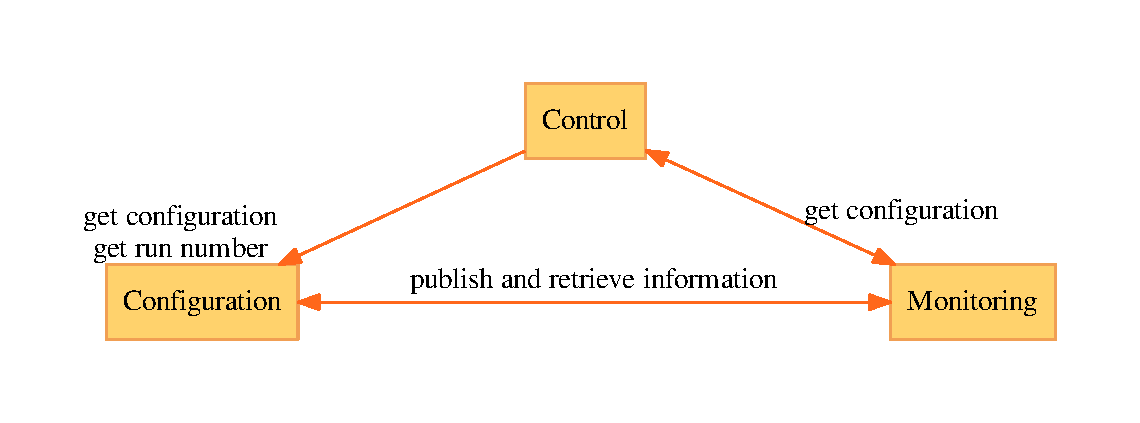
\includegraphics[width=0.8\textwidth]{daq-ccm-subsys.pdf}
\end{dunefigure}

The three \dword{ccm} sub-systems interact and operate together to guarantee efficient data taking.  As shown in Figure~\ref{fig:daq-ccm-subsys}, the Control sub-system relies on the Configuration to know which components participate the DAQ instance, which policies to apply for resource management and error handling and uses the Monitoring in order to retrieve the status of DAQ components and detect any anomalies.

It shall be noted that, while the CCM system is instrumental to the definition of the data taking conditions, the conditions database, as well as the definition of which conditions are important for offline analysis are not part of the CCM. The CCM will provide any required information in response to network requests.

\subsubsection{Control}
\label{sec:daq:design:ccm:control}

The DAQ Control sub-system is composed of a number of functional blocks in global or partition scope as illustrated in Figure~\ref{fig:daq-ccm-control}. 
Those blocks shown in partition scope have instances created for each partition. 

\fixme{I (bv) redrew this from Giovanna's to get vector PDF and match DUNE color palette.  I made two content changes: 1: move UI out of partition as it can't both initiate a partition and be inside it and likely will allow for creation/viewing of more than just one partition.  2: I had to guess on how garbage collection might go and so addded a line from RM to PM. }

\begin{dunefigure}{fig:daq-ccm-control}{Roles and services which compose the DAQ Control sub-system.}
  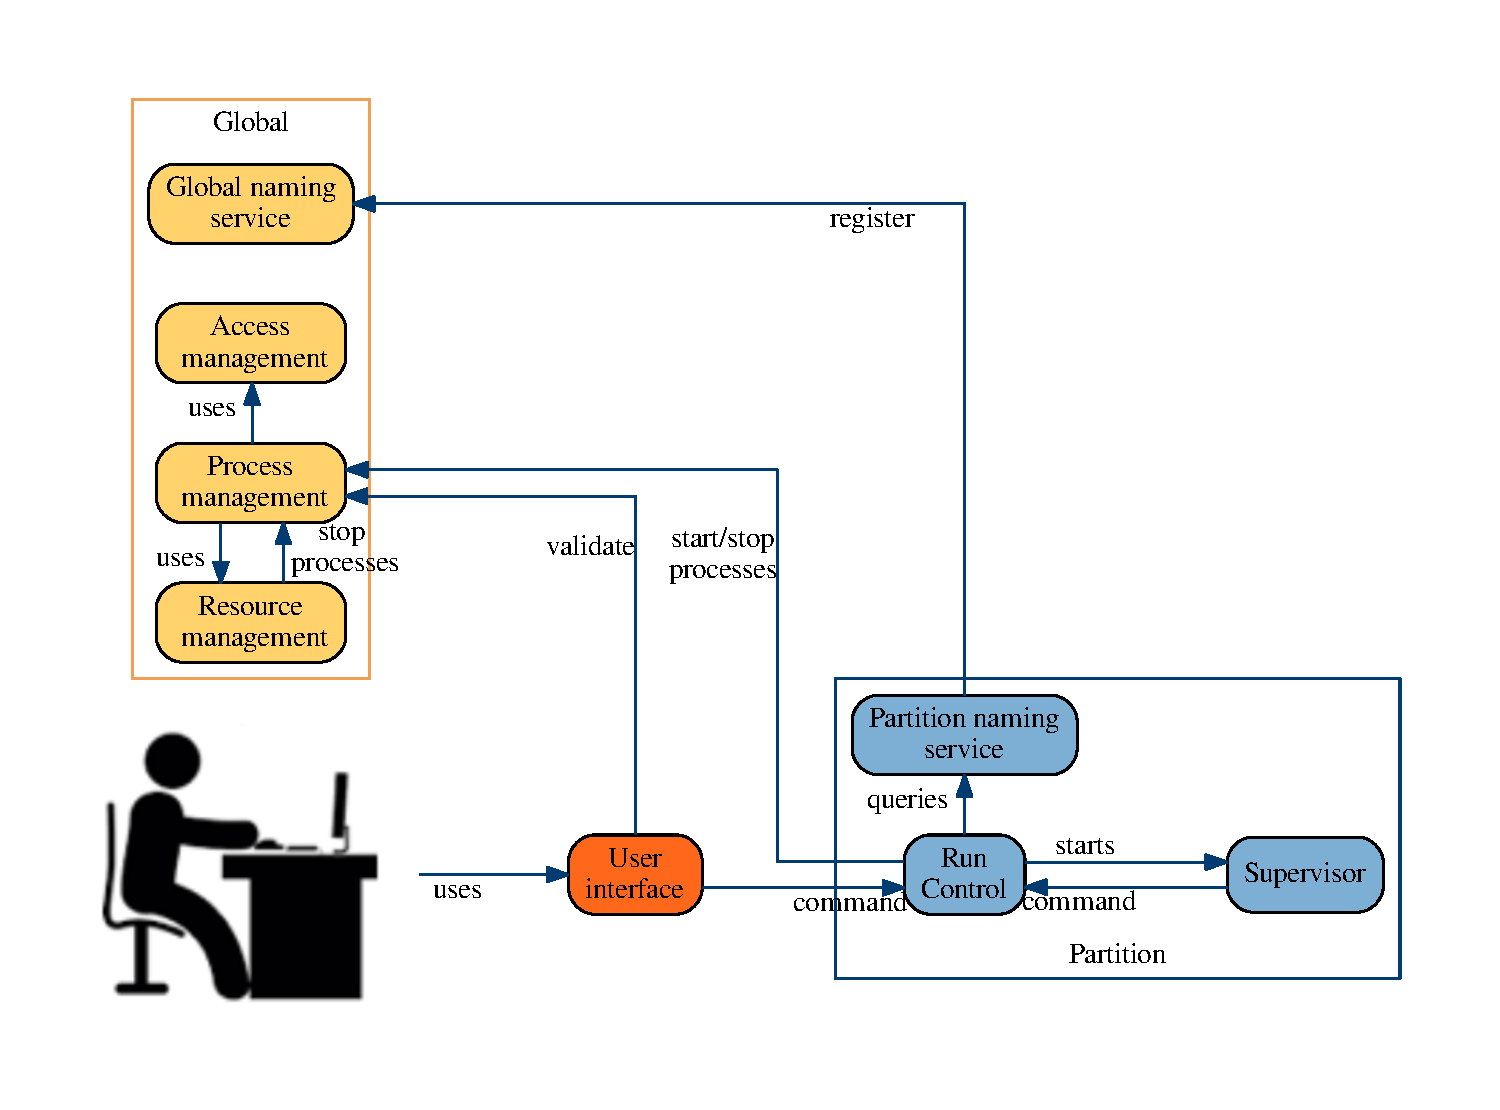
\includegraphics[width=0.8\textwidth]{daq-ccm-control.pdf}
\end{dunefigure}

The functional blocks represent one or more semi-autonomous and redundant agents each with defined roles, capabilities and access.  First the blocks at partition scope are described.

\begin{description}
\item[Partition naming service] This block provides \dword{daqdispre} at the scope of one \dword{daqpart}. 
  The block provides a mechanism for a component in the partition to learn of the existence of others, their identities as well as determine if they are currently operational or have become unresponsive.

\item[Run control] Starting a \dword{rc} block is the first step toward initiating a \dword{daqpart}. 
  The \dword{rc} shall accept, interpret and validate input commands.  The commands shall describe the desired initial state of the aggregate of all components which are to comprise the \dword{daqpart}.  \dword{rc} may query other blocks to perform validation and then shall execute the commands by allocating processes through Process management.  Once successfully allocated, their lifetime is managed by \dword{rc}.  Throughout their lifetime \dword{rc} may reconfigure existing processes, destroy them or allocate additional processes.  \dword{rc} may query the Partition naming service to resolve resource identifiers referenced in commands to network endpoints.  

\item[Supervisor] The initiation of a \dword{rc} block shall coincide with the initiating of a Supervisor block.  This block shall augment human commands with automated ones such as those needed for \dword{rc} to initiate actions to recover from some exception.

\end{description}

Global scope controls DAQ components for all \dwords{daqpart} across all \dword{fd} modules\footnote{DAQ instances at locations other than the \dword{fd} cavern are expected to be wholly distinct.}.  It consists of the following blocks.


\begin{description}
\item[Global naming service] This role aggregates the \dword{daqdispre} information across the partitions and in particular regarding the \dword{rc} instances.

\item[Process management] This role allocates and may reclaim sets of processes on behalf of a requesting component (specifically \dword{rc} and Resource management). 
  An allocation request shall include a complete description of the processes and their initial configuration information. 
  A successful allocation shall occur only after this role initiates all processes and confirms their presence. 
  Process management shall only allocate if the requester has sufficient access privileges as determined by Access management and if sufficient resources exist as determined by Resource management. 
  Process management may support pre-allocation where sufficient access is determined and resources are confirmed and reserved and a token (``cookie'') is returned to the requester. 
  This cookie may be presented to complete the allocation and claim the processes. 
  After a configured timeout period the cookie may be invalidated.\footnote{This will be required if the race condition between multiple UIs and RCs is a problem.}  
  
\item[Resource management] This role shall determine if any process allocation may proceed and provides process garbage collection. 
  Resource management shall monitor the presence of all successful allocations as well as that of their requester.  
  An allocation shall be accepted only if the resulting aggregate of processes violate no constraints maintained by Resulting management.
  Resource management shall notify Process management of any remaining processes from an allocation when it detects that the requester has ceased to assert presence.
  This role shall also support allocation pre-validation queries. 
  The response to shall indicate whether the allocation would succeed at the current time but such a query shall not be interpreted as an allocation. 
  No guarantee may be provided that the allocation may succeed or fail if subsequently requested.

  
\item[Access management] This role is responsible for providing authentication and authorization for all DAQ functions which require access control.  

\end{description}

The last block in Figure~\ref{fig:daq-ccm-control} represents applications which shall provide user interfaces (UI) to the Control sub-system which shall be developed to allow a trained operator to construct and issue commands required to initiate, configure, potentially reconfigure and finally terminate \dwords{daqpart}. 
The UI may validate user commands prior to issuing them to an \dword{rc} by directly querying the process manager block. 
If sufficient resources are currently unavailable or if the user lacks sufficient access the response shall include a descriptive error which the UI shall present to the human.
If validation passes the UI shall send the command to the \dword{rc} for execution. 
Additional UI elements shall be developed as described in Sections~\ref{sec:daq:design:ccm:configuration} and~\ref{sec:daq:design:ccm:monitoring}.


\subsubsection{Configuration}
\label{sec:daq:design:ccm:configuration}

The DAQ Configuration sub-system shall a persistent data store for all historic, current and potential future configuration information applicable to the DAQ.
Further, it shall maintain a record of the use of any configuration for every \dword{daqrun} and it shall provide for allocation of unique \dwords{daqrunnum}. 
All data stores shall be insert-only and shall not support updating or deletion of existing records.
The stores shall support the following types of information.

\begin{description}

\item[Partition structure] shall contain descriptions of the multiplicity and connectivity of DAQ components for any partition which has or may be formed. 
  Structure shall be expressed in an abstract manner and ultimately in terms identifiers associated with logical addresses of detector electronics. \footnote{Mapping from abstract to concrete addressing may be done through the discovery and presence provided by naming services described in Section~\ref{sec:daq:design:ccm:control}.}

\item[Component parameters] shall contain descriptions of configuration parameter sets associated with any DAQ component that has or may be initiated.  It shall accommodate data schema specific to each type of component. 

\item[Run number] shall provide a sole source atomic allocation of unique, monotonically increasing \dwords{daqrunnum}.

\item[Partition instances] shall provide a record, associated with a run number, of the partition structure and set of component parameters used to initiate a \dword{daqpart} or applied to a subsequent reconfiguration.  Records may consist of references into the subsequent stores.

\item[Constraints] shall provide definitions of all constraints that have been or may be considered by Resource management. 
  It shall record which constraint was employed by Resource management over time.
\end{description}


All stores provided by the Configuration subsystem shall provide a redundant access mechanism that assures any other requirement such as atomic run number allocations. 
The access mechanism may be provided as a layer between client access and store implementation.
For stores of data structures of complexity prohibitive to manual construction configuration editors and generators shall be developed.

backups, offsite replication


\subsubsection{Monitoring}
\label{sec:daq:design:ccm:monitoring}

The DAQ Monitoring sub-system is intended assist humans and expert systems in the detection, diagnosis and correction of anomalous activity, observation of intended operation and provide a historical record.
It shall accept the required information produced by any DAQ component (here called ``status'').
Status shall be stored a period not less than that required for the corresponding detector data to undergo initial offline data quality validation.
Status shall be made available in a form suitable for human understanding promptly. 
The required latency defining promptness needs further study and is expected to vary depending on the type of status and the purpose of its consumption.  
Status shall be retrieved based on the time it was produced and the logical and physical addresses associated with its producer.
This may be satisfied by developing status views accessing the status stores or it may be provided by views which subscribe to one or more of the status feeds provided by individual components.

The precise implementation of the production, acceptance, store, post-processing, querying, visualization of monitored status requires additional development. 
However, the selected \textit{linuga franca} IPC system described in Section~\ref{sec:fd-daq:design-messages} shall be used to deliver status information to the Monitoring sub-system. 
Where this may conflict with a native IPC used by some subsystem a proxy may be supplied. 

In general, the \dword{pubsub} network communication pattern shall be followed. 
The Monitoring system may be further decomposed into a number high-level IPC protocols which are specified in terms of their message types and schema and the behavioral expectations at either endpoint of a connection.
These are categorized as:


\begin{description}
\item[Common] all protocols shall have commonalities in terms of message identifiers including: \dword{pubsub} topic, sub-protocol type, message type, sender, host computer time and where applicable associated detector data time.  Specific protocols extend this by providing additional ``payload'' to their messages as described in the following items.
 
\item[Logging] payload consists of an integer determining subjective importance (eg, enumerating categories: debug, info, warning, error, fatal) and a succinct, human-readable information string providing explanation of what led to the occurrence including static type and variable information. 
\item[Metrics] payload consist of message in structure schema and carrying specific information about predefined aspects of the sender.  This is much like logging but the messages support automated consumption by expert systems.  
\item[Quality] payload consists of summary information derived from the detector data (eg waveforms) or its metadata (eg timestamps, error codes) while it is in flight through the DAQ.
\end{description}

Some status feeds accepted by the Monitoring sub-system may be processed and only the resulting data sent to permanent store. 
In particular the quality stream data rate may be prohibitively excessive so as to disallow long term storage in forms that meet the query requirements given above. 
For example, this stream may be summarized into histograms or other statistical representations which shall be saved while the full input quality stream shall be discarded.

In addition to this DAQ \dword{ccm} Monitoring sub-system there is a separate system that shall be used monitoring the quality of the content of the detector data itself.  See Section~\ref{sec:fd-daq:design-data-quality} for its description.

\subsubsection{Partition Lifetime}
\label{sec:daq:partition-lifetime}

The partition lifetime is described here in a somewhat linear narrative but it must be stressed that the components shall not rely on any strict inter-component synchronization that is not explicitly constructed through a suitable protocol. 
In particular, components shall be robust to the order in which peers are discovered.

After the partition's processes are started through the allocation mechanism described in Section~\ref{sec:daq:design:ccm:control}, each component shall apply its initial configuration. 
This information shall include any personal identifiers the component will assert as part of \dword{daqdispre} as well as the identifiers required to locate any other partition components required to bootstrap its own operation. 
In particular, components shall be provided the identity of the partition's \dword{rc} instances so that it may take directives.

The central directive the shall observe involves receiving and subsequent configuration which is used to construct the overall partition structure and connectivity.  
This mechanism shall enable \textit{zero-downtime reconfiguration} as described next.
The partition components shall accept and enact a \textit{configuration change command} (CCC) received from their identified \dword{rc}. 
A CCC shall provide at least the following pieces of information:

\begin{description}
\item[run number] is a globally unique integer drawn from a monotonically increasing sequence managed by the DAQ Configuration sub-system as described in Section~\ref{sec:daq:design:ccm:configuration}. 
  the \textit{run number} identities the instance of the partition as a collective whole which is to be constructed by the CCC that have been distributed.
\item[activation time stamp] (ACT) states the \textit{data time} (see Section~\ref{sec:fd-daq:design-messages}) at which the CCC shall take effect. 
\item[configuration payload] provides the component-specific configuration to be enacted and may include  pre-ACT actions that shall be made to assure a zero-downtime transition.
\end{description}

Upon receipt, a component shall create any new connections to peers and enact any other pre-ACT actions as directed by the CCC and it shall begin (or continue) to monitor the \textit{data time} of received messages. 
If the component was operational prior to the receipt of the CCC as part of an earlier partition it shall continue its otherwise normal operations until the ACT is reached. 
Upon receiving input containing a \textit{data time} at or after the ACT it shall apply the new configuration specified in the CCC. 
At this point, any pre-ACT data which may be buffered by the component shall be flushed to its output. 
Any input or output connections which are no longer applicable for the new partition definition shall be dropped. 
Finally, the component shall renew operations starting with the data passing the ACT threshold and which initiated the reconfiguration.

In order for this mechanism to truly provide zero-downtime reconfiguration the CCC messages must be received by the partition components sufficiently in advance of input data passing the ACT time.
This requires the human-UI-\dword{rc} chain to select an ACT with knowledge of recent \textit{data time} and typical latency of the mechanism. 
It is expected that a lead time of on order 1-10s is required. 

After cycling through zero or more run numbers, the partition may be terminated. 
Termination shall be initiated by the partition's \dword{rc} issuing a final round of CCCs. 
As above these shall instruct the components to continue processing until the ACT is reached and after which any buffers shall be flushed to output. 
Unlike zero-downtime reconfiguration the component shall then destroy all connections and exit. 
The \dword{rc} shall notify the UI and Process manager of this destruction of the partition (saving briefly the \dword{rc} itself). 
The Process manager shall forward to the Resource manager that the resources have been released. 
The \dword{rc} shall then itself terminate and the partition is no more.
The Resource manager shall confirm partition processes have terminated through \dword{daqdispre}. 
In the exceptional case that the \dword{rc} aborts without cleanly terminating the partition its absence shall be detected and the remaining partition processes shall be reaped through the garbage collection mechanism described in Section~\ref{sec:daq:design:ccm:control}.

\subsubsection{Self-healing}
\label{sec:daq:self-healing}

The above zero-downtime reconfiguration mechanism is intentional and typically driven by human action or via automated run sequencing algorithms. 
In a similar manner, the partition shall \textit{self-healing} in the face of unexpected failures that render peers unresponsive or when unexpected information content is received by partition components.  
Extending the metaphor, self-healing involves these phases: \textit{detection} of an injury to the partition, \textit{diagnosis} of the scope of the injury and \textit{intervention} by executing an action on the partition.

Detection shall be performed by the DAQ Control sub-system Supervisor functional block in at least one of two methods.
First, if a partition component become unresponsive (ie it ``crashes'' or ``hangs'') the Supervisor shall receive notification via DAQ \dword{daqdispre}. 
Second, if a partition component detects injury such as receiving unexpected data it shall report the occurrence via IPC to the Supervisor.

Upon any detection the Supervisor shall determine which partition components are impacted.  The heuristics and methods to perform this diagnosis may evolve as failure modes are discovered and/or removed.  The 

Finally, the Supervisor shall respond to the detection. 
Response shall in all cases include notifications to the Monitoring sub-system. 
Any addition response is in the form of sending commands to the \dword{rc} to initiate a reconfiguration or a termination. 
When initiating a reconfiguration, as with any, the command to the \dword{rc} shall include information required by the \dword{rc} to issue CCC messages. 
As a consequence, the partition shall be reconfigured (and thus begin a new run number) as described in Section~\ref{sec:daq:partition-lifetime}.


\subsection{Detector Readout}
\label{sec:fd-daq:readout}
\fixme{module-generic}
\fixme{Add words on the Data Selectors which front the Buffer.}

The Readout system shall be the first DAQ element in the data flow chain of the DAQ system.
Conceptually, this system corresponds to the receiver, buffer and a portion of the trigger subsystems illustrated in Figure~\ref{fig:daq-conceptual-overview}.
It is physically connected to the detector electronics via optical fiber and buffers and serves data to other DAQ sub-systems, namely the Data Selection and the Event Builder as detailed in Figure~\ref{fig:daq:readout}.\fixme{It would be nice to redraw this using DUNE colors.}

\begin{dunefigure}{fig:daq:readout}{DUNE DAQ Readout system and its connections.}
  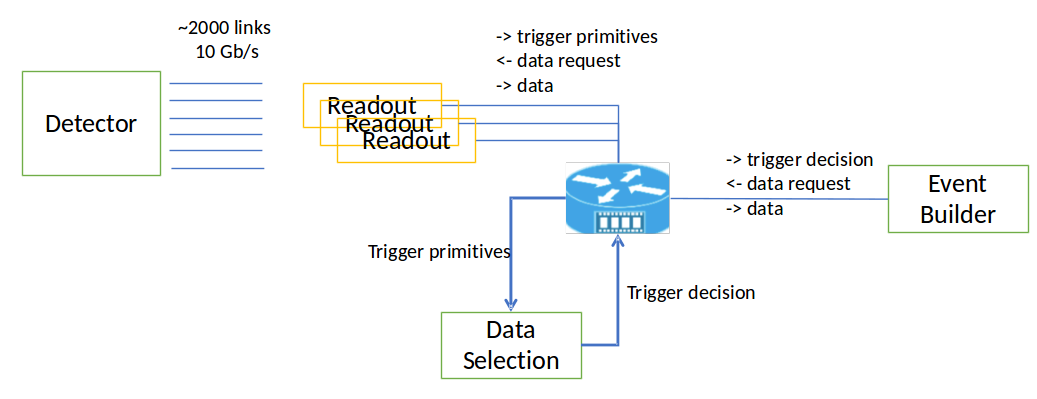
\includegraphics[width=0.8\textwidth]{daq-readout.png}
\end{dunefigure}

The Readout system is composed of many similar \dword{daqrou}, each connected to a sub-set of electronics from a detector module and interfacing to the DAQ switched network.  Each unit encompasses four functional blocks:

\begin{enumerate}
\item Data reception
\item Network based I/O
\item Data processing
\item Temporary data storage
\end{enumerate}

Each of these facets are described below.  In addition and like all other DAQ sub-systems, the readout participates in the common software framework for control, configuration and monitoring as described in Section~\ref{sec:fd-daq:design-run-control}.

\subsubsection{Data reception}

The physical interface between the detector electronics and the DAQ for the purpose of data transmission are 10 Gbps point-to-point serial optical links, running a simple (e.g. 8/10 bit encoded) protocol. 
The number of links per DUNE module vary from about 1000 to 2000, depending on the adopted detectors technologies.

In order minimize the space and power consumption footprint of the DAQ, 10-20 links are aggregated into \dword{felix} boards hosted in \dword{cots} computers. 
\dword{felix} is an FPGA-based PCIe board developed initially for ATLAS and now proposed or in use in a number of experiments including ProtoDUNE. 
Existing firmware shall be adopted and adapted to ensure decoding and format checking of the incoming data and to then marshal the data to the other blocks of the readout sub-system.

\subsubsection{Network based I/O}

The Readout system shall provide access to the data selection and back-end egress systems through a \dword{cots} switched network as illustrated in Figure~\ref{fig:daq:readout}).
The network communication protocol shall be as described in Section~\ref{sec:fd-daq:design-messages}.
The network I/O shall be handled by the \dwords{daqrou} via software and in particular, dedicated hardware or firmware development is not required.

\subsubsection{Data processing}

The data processing functional block is in charge of the identification of active areas in the detector (in the TPC and photon detection systems) as a function of time.

As a preliminary step data may be pre-processed, i.e. organized in the way that best suits the subsequent data analysis. This may imply reorganizing data into different streams, applying noise filtering algorithms, compressing and/or zero-suppressing data.

The identified detector activity (aka ``hit finding'') is summarized by the Readout system into so-called trigger primitives that are forwarded to the Data Selection system, to make correlations and take a decision on whether and which data shall be saved.

This functional block may be implemented onto FPGAs, GPUs, CPUs or in a mixed fashion. A decision on the implementation is premature at this stage and this is one of the main R\&D topics to explore in the Readout area.

\subsubsection{Temporary storage}

In DUNE, the Readout system is in charge of storing the data until the Data Selection system has formed a decision and such that the Egress system may have sufficient time to request and receive the corresponding data.
There are a number of time scales and data throughput which dictate the technology and its scaling which is required to satisfy these requests.

The first is driven by the predominant physics which produces visible activity promptly after interaction and compactly in space and time. 
The latency to form a trigger condition in this case is dominated by processing speed and pipeline depths and is expected to be on order of one second.  The amount of data which is expected to be requested as a result of such decisions is on order one or two TPC drift times (5-10\si{\milli\second} depending on detector technology).

On the other hand the very rare but important case of a potential \dword{snb} has substantially different and more stringent requirements. 
Potentially many seconds of activity may occur which is too infrequent and low energy to form a trigger decision but which can have important physics information. 
In order to capture that, when a \dword{snb} decision is formed the DAQ shall record at least the prior 10 seconds of data. 
\dword{snb} occurrences are so important that all data shall be recorded over their expected duration. 
To satisfy that, the DAQ shall record a minimum of 30 seconds of data from a \dword{snb} trigger decision. 
The data rates and volumes involved in satisfying these requirements are such that different technology and scale must be employed compared to that required to select data from compact interactions.

The worse-case temporary storage requirement for the readout system (using single phase detector technology as a metric) is in the order of 100 TB per DUNE detector module, with a throughout of approximately 10 Tb/s.
This figure is challenging, but technically achievable already with today's technologies, with a suited granularity of the \dwords{daqrou}. 

It is expected that in this area requirements will still be refined during the detailed design phase of the DAQ system, taking into account the ability of partially compressing data as well as more realistic estimates on trigger decision latency, etc.


% \metainfo{Describe how FELIX hardware defines an interface which common to all modules.  Describe how the hardware may handle UDP or other prototocols including bidirectional communication.  Describe how FELIX can be scaled to accept data across a spectrum in order from large to small data rate: the full SP data from the WIBs, full compressed data from the DP, trigger primitive stream from FPGA based units placed between WIBs and FELIX.}


% \ifdp
% \subsubsection{DP data ingest via UDP}
% \label{sec:dp-daq:design-udp-ingest}
% \fixme{dual-phase module, move to DP-DAQ chapter eventually}
% \metainfo{This is a DP section and will be only in the DP volume. 
%   It should describe the ``Bump On Wire'' from the IDR unless we can
%   come up with any new/better ideas.}
% \metainfo{Include full hardware scope starting at fibers from CE and
%   ending at the output of trigger processors and the interface between
%   buffer and the Data Selector.
%   Describe the per-APA multiplicity of computers, CPU cores, host
%   system RAM, host system storage, FELIX boards, DPM components (RAM,
%   SSD). 
%   Include thermal estimates itemized by components.}  
% \fi

% \subsection{Front-end Data Handling and Processing}
% \label{sec:sp-daq:design-fe-processing}

% \metainfo{This section describes four functional blocks: (1) 10s RAM buffer (minimum), (2) non-volatile SNB buffer for 30s of data once per month (minimum), (3) hardware for the production of trigger primitive including any data formatting and DPS filtering and (4) compression of selected data.  Note, actual algorithms for trigger primitives are described in Section~\ref{sec:sp-daq:design-selection-algs}.}

% \metainfo{One or two sentences that positions the two processing
%   patterns (FEDHP either before or after FELIX) in this section as options. 
%   Say that the ``FPGA before FELIX'' option is used for ``baseline costing''.}

% \metainfo{Include a table with one row for each known compression factor: protoDUNE RCE and FELIX, MicroBooNE before and after noise filter (see docdb), 35t, protoDUNE data after ADC stuck code mitigation or avoidance, simulations.  One column of this table shall give a brief comment of how it applies to DUNE including any caveats or reasons for over/under estimation.}

% % \subsubsection{FELIX+FPGA}
% \subsubsection{Upstream FPGA and Firmware}
% \label{sec:sp-daq:design-felix-fpga}
% \fixme{single-phase module}

% \metainfo{Include full hardware scope starting at fibers from CE and
%   ending at the output of trigger processors and the interface between
%   buffer and the Data Selector.
%   Describe the per-APA multiplicity of computers, CPU cores, host
%   system RAM, host system storage, FELIX boards, DPM components (RAM,
%   SSD). 
%   Include thermal estimates itemized by components.}

% % \subsubsection{FELIX+CPU}
% \subsubsection{Downstream CPU and Software}
% \label{sec:sp-daq:design-felix-cpu}
% \fixme{single-phase module}

% \metainfo{Include full hardware scope starting at fibers from CE and
%   ending at the output of trigger processors and the interface between
%   buffer and the Data Selector. 
%   Describe the per-APA multiplicity of computers, CPU cores, host
%   system RAM, SSD and FELIX boards. 
%   Include thermal estimates itemized by components.}


% \subsubsection{Photon Detection System Interface}

% \metainfo{Some motivations for using light to trigger. 
%   (1) want to understand PDS so want to trigger on just the PDS. 
%   (2) background to SNB for which PDS trigger primitives may eliminate. 
%   (3) possibly must rely on light only for SNB triggering, eg if noise is out of control. 
%   Some to all of these should be included.}

% \metainfo{Possibly want to \SI{1}{\micro\second} packet for every time a 1-PE threshold is crossed. 
%   PDS is still understanding what they may send. 
%   DAQ needs to be in control of the trigger forming.}

% \ifdp
% \subsubsection{DP TPC FE issues}

% \fixme{dual-phase module}

% \metainfo{This is similar to SP except for the need to decompress before any trigger primitive processing.  Decompression can potentially happen on FELIX FPGA or on CPU.  There shall be a table or description of the amount of processing required.}

% \subsubsection{DP SP Issues}
% \fixme{dual-phase module}
% \fi

\subsection{(empty)}

\fixme{This section was merged with above and should be removed.  Leaving it in temporally to not confuse numbered writing assignments.}


\subsection{Data Selection}
\label{sec:sp-daq:design-selection-algs}
\fixme{single-phase module}

\fixme{There are many studies which could go into this section. Some of this may very likely be moved into one or more tech notes and referenced.}

The Data Selection sub-system (DS) is responsible for real-time processing
of data from all detector subcomponents; based on processing
outcomes and external inputs, it is responsible for making decisions
about what data must be transferred to the Backend System, and
distributing those decisions to the Egress sub-system. Data processing
is executed in various stages of firmware and/or 
software, and the overall sub-system is designed in such way as to
provide flexibility on where the core processing payload functionality
resides (hardware, firmware, or software). 

A key sub-system requirement is to select data associated with beam
interactions, atmospheric neutrinos, rare baryon number violating events,
and cosmic ray events depositing visible energy in excess of 100 MeV
with $\gt$99\% efficiency. A second key requirement is to select data
associated with potential galactic supernova bursts. This implies that
the data selection sub-system must be capable of self-triggering on
supernova bursts with $\gt$95\% efficiency. In order to also keep with the
requirement that the DUNE FD maintain a $\lt$30~PB per yr to permanent
tape, the DS sub-system must effectively reduce the generated data
volume by four orders of magnitude, and maintain a fake supernova
burst trigger rate of less than 1 per month.

The DS sub-system design follows a hierarchical level structure, where low-level
decisions and forward-fed into higher-level ones, ultimately
determining the issuing of a  module-level ``trigger''. The hierarchy
structure is illustrated in Figure~\ref{fig:daq:data-selection}. The hierarchy structure
consists of four levels of processing: Trigger Primitive Generation;
Trigger Candidate Generation; Module Level Trigger; and High Level
Trigger. Each are described in subsequent sections.

\begin{dunefigure}{fig:daq:data-selection}{Block diagram of DUNE DAQ
    Data Selection sub-system, illustrating hierarchical structure of
    sub-system design.}
%  \includegraphics[width=0.8\textwidth]{daq-data-selection.pdf}
\end{dunefigure}

Two general classes of trigger decisions are envisioned for the first
stage of operations:
\begin{itemize}
 \item Localized (in time and space) activity triggers: These are
   low-latency triggers and are intended to prompt readout of
   high-energy events (depositing $\gt$100~MeV of visible energy) 
   and potentially also low-energy events
   (e.g. from solar neutrino interactions). In association with a
   localized trigger, a total of 5.4 ms worth of data is recorded from
   the entire 10-kton module that generated the trigger, including
   both TPC and PDS subsystems.   
\item Extended (in time and space) activity triggers: These are
  high-latency (up to 10 seconds) triggers and are intended to prompt readout of
  supernova burst-associated activity. This activity spans multiple
  tens of seconds and comprises multiple supernova neutrino
  interactions as part of a $\sim$10-second burst (from ~a few to
  ~thousands of interactions in the case of a galactic supernova
  burst). In association with an extended trigger, a total of 30-100
  seconds worth of data is recorded from the 10-kton module that
  generated the trigger, including both TPC and PDS subsystems, as
  well as from the other three 10-kton modules, regardless of whether
  the latter have generated an extended trigger of their own or not.  
\end{itemize}

To facilitate partitioning, the Data Selection sub-system must also be
informed and aware of detector configuration and conditions in real
time, and apply certain masks on subdetectors or components
in its decision making. It is also required to provide to the Egress sub-system a list of
subcomponents to read out, in association
with any module-level trigger.

\subsubsection{Trigger Primitive Generation}
\label{sec:sp-daq:design-trigger-primitives}
\fixme{single-phase module}

A Trigger Primitive is defined nominally on a per-channel basis, and,
in the case of the SP TPC, it is identified with a per-collection-wire
``hit''. Trigger Primitives provide summary information
such as the start time of the pulse on a collection wire, the total
charge or peak of the collection-wire pulse, and the time the pulse
stays above some pre-determined threshold. Trigger Primitives for the
TPC are generated in the front-end readout part of the DAQ 
system, either in FPGA firmware, or in CPU or GPU software. For the
PDS, TPs are generated in the PDS hardware and streamed to the DAQ
DS sub-system.

Algorithms for trigger primitive generation are under continuing development
\cite{docid-11275}. An example algorithm is one which a priori establishes
channel baseline, applies baseline subtraction and thresholding, and
identifies a hit over threshold \cite{docid-11236}. This algorithm has been
validated with both Monte Carlo simulations and real data from protoDUNE. The performance is
summarized in Section~\ref{sec:sp-daq:design-validation}.

Each trigger primitive consists of the following information:
\begin{itemize}
\item channel address \[32 bit\]
\item time of hit \[64 bit\]
\item time over threshold \[16 bit\]
\item ADC sum \[32 bit\]
\item error flag \[16 bit\]
\end{itemize}
corresponding to a total of 20 Bytes.

The anticipated trigger primitive rate  is expected to be dominated by
$^{39}$Ar rates (10 MHz per module). Assuming the above TP format
prescription, the anticipated trigger primitive rate is expected to be
200 MB/s . The subsequent stage of the DS must be able to absorb and
process this TP rate in real time, providing Trigger Candidate decisions. 

\metainfo{Include plot and discussion of DUNE trigger primitive rate in protoDUNE. 
  The fact that this includes many more cosmics will not matter much as the rate is expected to be dominated by Ar39. 
  Phil has this already but the LAr purity is not yet high enough to see Ar39 across the whole drift distance.}

\subsubsection{Trigger Candidate Generation}

Trigger Primitives are streamed from the front-end DAQ readout to a
higher level of data selection which examines those on a per
subdetector (e.g. per APA) basis. This higher level of data selection examines
whether the Primitives from that subdetector constitute a potential
Trigger Candidate. Trigger Candidates are generated by looking for
clusters of multiple hits in a narrow time window, the total ADC sum of one or a
cluster of hits, or a large time-over-threshold. Trigger 
Candidates will be generated with both a “low” and “high”-energy threshold. The former
will be used for supernova burst triggering, the latter for triggers on beam, atmospheric
neutrinos, cosmics, and other high-energy interactions in the detector. 

A Trigger Candidate includes not only timing and subdetector
identifier information, but also a rudimentary estimate of the detector
activity which led to its formation, so that further downstream (at
the Module Level Trigger stage) a decision can be made on 
whether a particular Trigger Candidate should be counted as part of a possible supernova
burst, or a different type of trigger. For example,
a candidate with an estimated energy of 100~MeV would be considered a
localized high energy trigger, while
one with an estimated energy of 5~MeV would only be considered as potentially part of a
supernova burst.

\subsubsection{Module Level Trigger}
Trigger Candidates are passed upstream to a “Module Level Trigger'' that collects candidates
and makes the final decision on whether a valid localized high-energy
activity (necessitating a module-wide readout trigger for a relatively
short, 5.4~ms duration) has occured,
or a possible supernova burst (necessitating a module-wide readout
trigegr for a minimum of 30 seconds) has occured. The Module Level Trigger passes
Trigger Commands, via the Egress sub-system, down to the front-end DAQ
Readout, prompting the readout of a pre-determined amount of data depending
on the type of Module Level trigger that has occurred. 

The Module Level also takes inputs 
from an “External Trigger,” including information from other
modules, SNEWS alerts, and other external signals such as
calibrations, 
and it also sends information to the External Trigger so that other modules or
detectors can be triggered.

\subsubsection{High Level Trigger}

The last processing stage of the data selection sub-system is the High
Level Trigger, which resides in the
Back-end part of the DAQ, and is further described in Section~\ref{sec:fd-daq:design-data-reduction}. The High Level Trigger acts on events that have already been triggered, read out,
and built by the Event Builder, and it serves several purposes: It
serves to limit the total triggered data rate that goes to disk, by
applying more refined selection criteria that removes events that are clearly uninteresting. For example, instrumentally-generated events
(e.g.~correlated noise) might lead to Trigger Candidates and a Module
Level Trigger, but upon more detailed inspection those can be clearly determined
to be non-physics events. It can also serve to reduce the triggered
data set through further identification and localization of
interesting activity.

Beacuse the HLT is in the DAQ Back-end and operates on Event-built data, the rate
of which is expected to be low, developing more sophisticated
algorithms to eliminate empty APAs from the data 
stream is possible.

\subsection{Back-end System}
\label{sec:fd-daq:design-backend}
\fixme{module-generic}

The DAQ back-end system conceptually encompasses the egress subsystem and interfaces to the buffer and trigger sub-systems illustrated in Figure~\ref{fig:daq-conceptual-overview}. 
It accepts trigger commands produced by the Data Selection system as described in Section~\ref{sec:sp-daq:design-selection-algs}. 
It queries the front-end buffer interfaces and accepts returned data as described in Section~\ref{sec:fd-daq:readout}. 
Finally, it records the trigger command along with the corresponding selected data to the output storage buffer at which point data custody is transferred to the offline.

\subsubsection{Dataflow Orchestration}

In order to minimize data extraction latency, the back-end egress sub-system must not execute trigger commands to completion in a serial manner. 
This asynchronous execution is termed \dword{daqdfo} and shall operate in the following manner and as illustrated in Figure~\ref{fig:daq:backend}:

\begin{dunefigure}{fig:daq:backend}{Illustration of DUNE DAQ back-end operation.}
  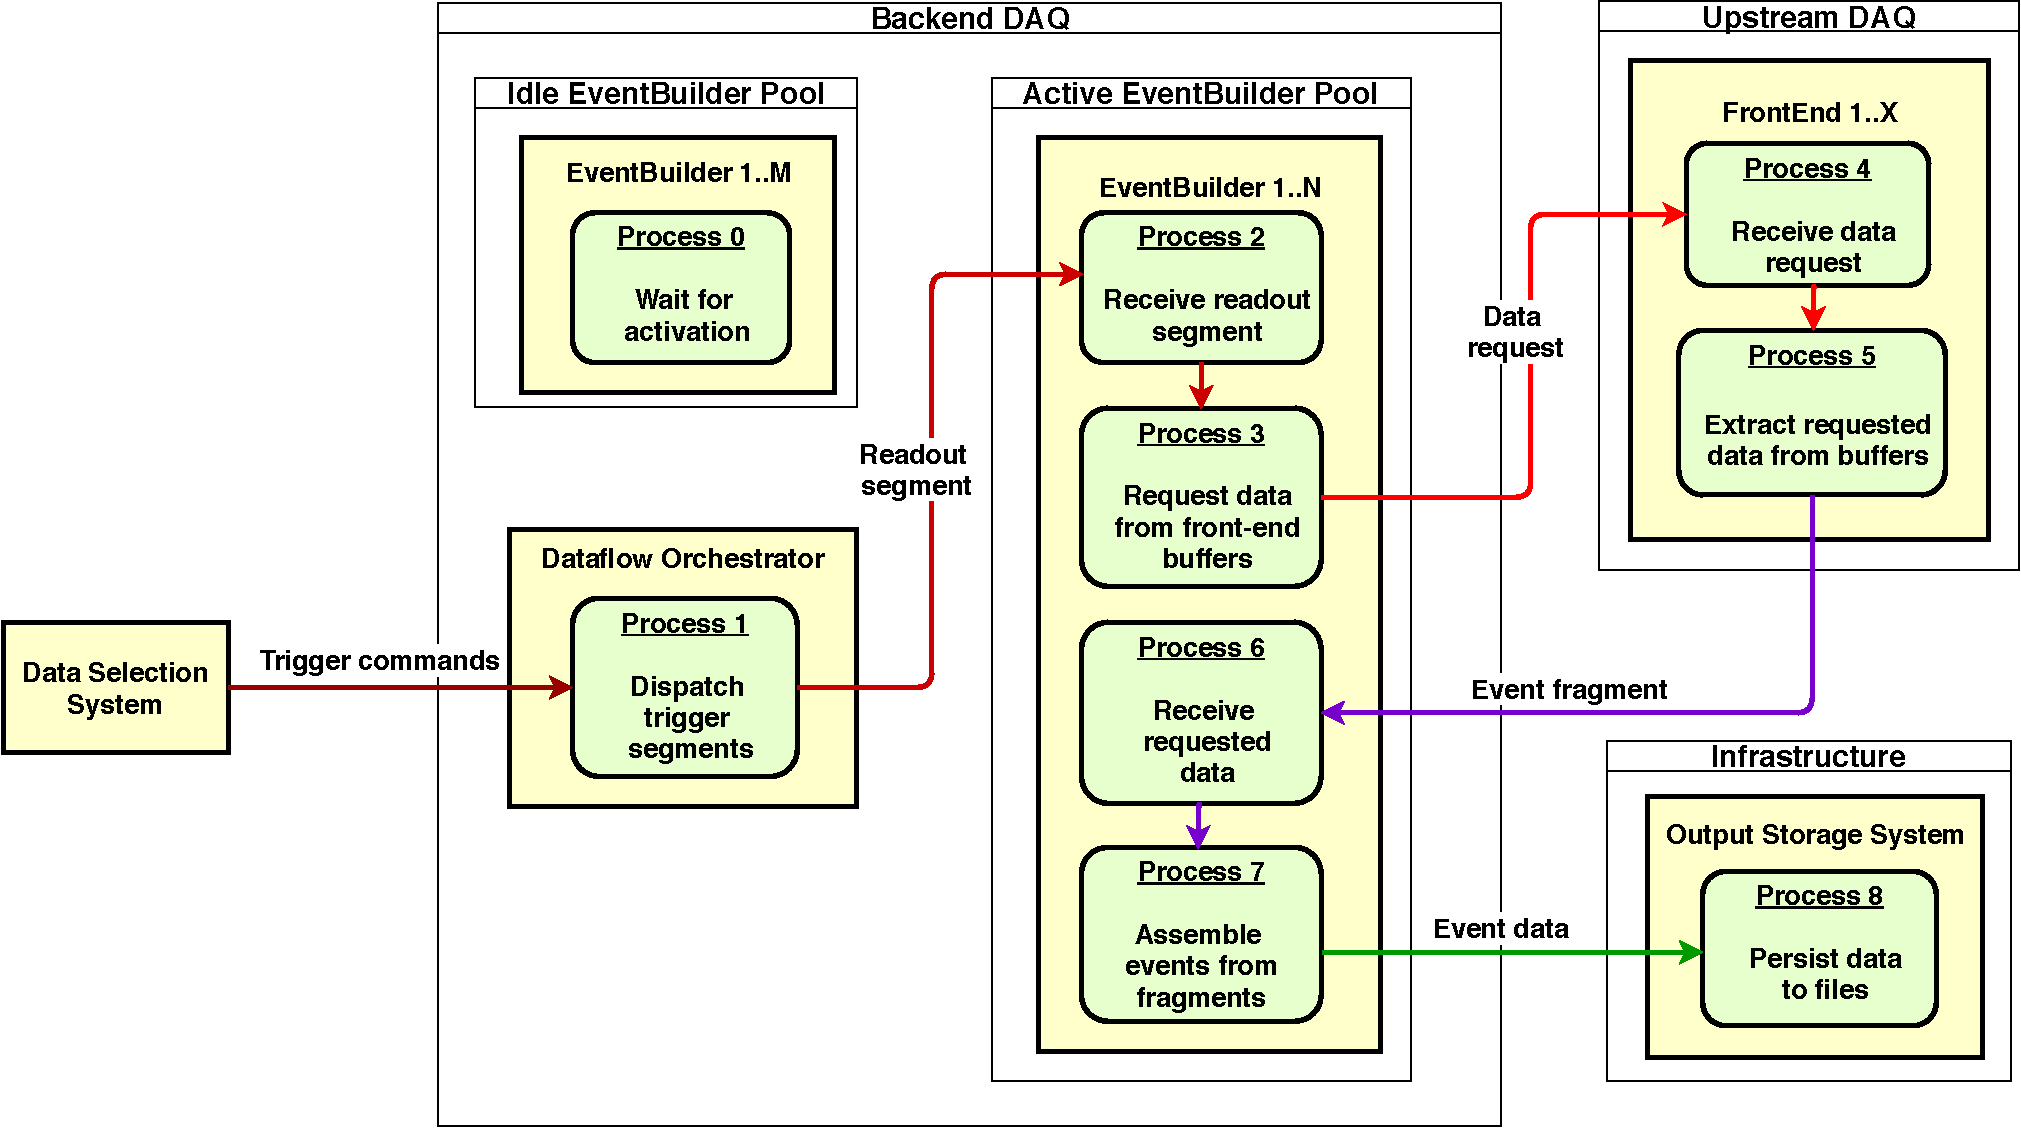
\includegraphics[width=0.8\textwidth]{daq-backend.pdf}
\end{dunefigure}

\begin{itemize}
\item \dword{daqdfo} shall accept a stream of time ordered trigger commands and shall dispatch each for execution.
\item It may evaluate the scope of a trigger command against a configurable set of constraints and segment it into multiple commands which contiguously and without overlap span the original command.
\item Each trigger command segment shall be dispatched to a process, termed an \dword{eb} and described in Section~\ref{sec:fd-daq:design-event-builder}, for execution.
\item \dword{eb} shall execute by requesting data covering the time period and detector span addressed by the trigger command segment.
\item Requests shall be made to the all associated \dwords{daqfbi} and the \dword{eb} may expect a response from all including if the buffer has already purged the requested data.
\item The returned data may undergo processing and further aggregation.
\item The returned data shall be saved to one or more files on the output storage system after which their custody is transferred to the offline.
\end{itemize}
\fixme{Add time order requirement on DS above}
\fixme{Add return-empty-response requirement to buffer above}



\subsubsection{Event builder}
\label{sec:fd-daq:design-event-builder}
\fixme{module-generic}

\metainfo{Explain artDAQ, handling of trigger commands by asynchronous, parallel queries to front end Data Selector (but take care not to duplicate between here and in the overview).}

The DAQ back-end subsystem shall provide instances of a process (\dfirst{eb}) which shall request data from each \dfirst{daqfbi} addressed by the consumed trigger command segment.  An \dword{eb} shall marshal the returned data to the output storage system.  It may apply addition processing of this data for the purpose of data reduction (Section~\ref{sec:fd-daq:design-data-reduction}) and quality monitoring (Section~\ref{sec:fd-daq:design-data-quality}) as the data are in flight. 
Resulting output files shall follow data schema and file formats as described in Section~\ref{sec:fd-daq:design-data-model}.


\subsubsection{L2 Data Reduction}
\label{sec:fd-daq:design-data-reduction}

To retain high efficiency for collecting activity of interest while minimizing selection and content bias as well as reducing output data rate it is expected that some high level data reduction processing may be required. 
This is termed second-level (L2) data reduction as it follows from the first-level provided by the Data Selection system as described in Section~\ref{sec:sp-daq:design-selection-algs}.
Simulation-based studies are expected to be performed during the lead-up to construction and initial data analysis after operation may also be required in order to fully understand the amount and type of data reduction which may be beneficial. 
The DAQ back-end sub-system thus shall allow for some form of L2 processing but its scale it yet to be determined. 
The back-end subsystem should facilitate development of processing modules in an offline context and their porting or direct application to the back-end processing system.



\subsubsection{Data Quality Monitoring}
\label{sec:fd-daq:design-data-quality}

Section~\ref{sec:daq:design:ccm:monitoring} described a monitoring system in the context of the \dword{ccm} sub-systems. 
Monitoring of the quality of the information held in the detector data itself is critical to promptly responding to unexpected conditions and maximizing the quality of the acquired data. 
A system for continuously processing a subset of the detector data and promptly providing summaries for human consumption shall be developed and is termed DAQ \dfirst{dqm}.
The exact suite of products is expected to evolve and the \dword{dqm} subsystem shall be designed to facilitate this evolution. 
As many software modules are expected to be developed in an offline context the \dword{dqm} subsystem shall facilitate their reuse when applied to the sample of detector data accepted by the sub-system.


\subsubsection{Data Model}
\label{sec:fd-daq:design-data-model}
\fixme{module-generic}

\metainfo{Describe the data model. 
  This isn't a strict schema just things like how various parts of the
  detector readout map to files, etc.}

\subsubsection{Output Buffer}

\metainfo{Describe the output buffer system, how it's shared with offline, data hand-off prototocols.  Responsibility scope (eg, who handles transfer to FNAL).}

The output buffer system is a hardware resource provided by the DAQ and operated by the DUNE offline effort. 
It has two primary purposes. 
First it decouples the operation of the DAQ in producing its contents from the operation of transferring its contents from the far site and to archive storage units and offline processing. 
Second, it provides local storage that is sized sufficient to allow uninterrupted DAQ operation in the unlikely event that connectivity between the \dword{fd} and the Internet is lost. 
Based on the very unusual occurrences of connectivity loss at major labs as well as \dword{fd} sites of other long-baseline neutrino experiments the output buffer shall provide storage capacity sufficient to retain one week of output given nominal data production rate. 
The maximum data production rate for the \dword{fd} is set to be \SI{30}{\peta\byte/\year}. 
Thus the output storage buffer must have a capacity of approximately \SI{0.5}{\peta\byte} to service the entire \dword{fd}.
\fixme{How to reference the 30PB/yr requirement?}




\subsection{Timing Distribution}
\label{sec:sp-daq:design-timing}
%\fixme{single-phase module}
%\fixme{Is it indeed still single-phase specific?}
%\metainfo{Hardware, consumers, links.}

All components of the far detector are driven with clocks derived
from a single GPS disciplined source, and all module components
are synchronized to a 62.5 MHz clock. In order make full use of the
information from the photon detection system (PDS), the common clock
must be aligned within a single detector unit with an accuracy of
O(1ns). In order to form a common trigger for supernova neutrino burst
(SNB) between detector modules, the timing between them must be
aligned with an accuracy of O(1ms). However, a tighter constraint is
the need to calibrate the common clock to universal time (derived from
GPS) in order to adjust the data selection algorithm inside an
accelerator spill, which requires an absolute accuracy of O(1$\mu$s).

The DUNE FD uses a development of the ProtoDUNE-SP timing
system, whose design principle is to transmit synchronization messages over
a serial data stream with the clock embedded in the data. The format
is described in \cite{docid-1651}. The timing system design is
described in detail in \cite{docid-11233}.

Central to the timing system are four types of signals:
\begin{itemize}
\item a 10 MHz reference used to discipline a stable master clock,
\item a one-pulse-per-second (1PPS) signal from the GPS,
\item an NTP signal providing an absolute time for each 1PPS signal, and
\item an Inter-Range Instrumentation Group (IRIG) time code signal
  used to set the timing system 64-bit time stamp.
\end{itemize}
The timing system relates its time counter onto GPS time by
timestamping the 1 PPS signal onto its own clock, and reading
the corresponding time in software in NTP time.

The timing system synchronization codes are distributed to the DAQ
Readout components in the CUC as well as readout components on the
cryostat via single mode fibers and passive splitters/combiners. All
custom electronic components of the timing system are contained in two
$\mu$TCA shelves; at any time, one is active while the other serves as
a hot spare. The 10 MHz reference clock and the 1PPS signal
are received by a single-width Advanced Mezzanine Card (AMC) at the
center of the $\mu$TCA shelf. This master timing AMC is a custom board
and is responsible for producing the timing system signals and encode them onto
a serial data stream. This serial datastream is distributed over a backplane to 
a number of fanout AMCs. The fanout AMC is an off-the-self board,
carrying two custom FPGA Mezzanine Cards (FMCs). Each FMC has four SFP
cages, where fibers connect the timing system to each detector
component (e.g. APA), or Direct Attach cables connect
to other systems in the CUC.

In order to provide redundancy, two independent GPS systems are used,
one with an antenna at the surface of the Ross Shaft, and the other
with an antenna at the surface of the Yates Shaft. Signals from either
GPS are fed through optical single mode fibers to the CUC, where
either GPS signal can act as a hot spare while the other is active. 

\subsection{Design Validation and Development Plan}
\label{sec:sp-daq:design-validation}
\fixme{single-phase module}

\metainfo{One sentence to describe our validation strategy: exploit
  ProtoDUNE, use simulation and develope vertical slice tests. 
  Put each validation study (performed or future) in a subsubsection
  and describe either \textbf{how it justifies a decision} or
  \textbf{how its outcome will be used to make a decision in the
    future}.}

\subsubsection{FELIX Throughput Demonstration at ProtoDUNE-SP}
\label{sec:sp-daq:validation-pdune-felix}
\fixme{single-phase module}

\metainfo{Describe how the FELIX DAQ at ProtoDUNE-SP demonstrates a
  FELIX+CPU approach. 
  Describe the elements that are same or similar (full-rate to host
  RAM buffer) and different (higher-rate but external trigger).}


\subsubsection{RCE Throughput Demonstration at ProtoDUNE-SP}
\label{sec:sp-daq:validation-pdune-rce}
\fixme{single-phase module}

\metainfo{Describe how RCE DAQ at ProtoDUNE-SP demonstrates an FPGA
  approach with DUNE.}

\subsubsection{Trigger Primitives in Software}
\label{sec:sp-daq:validation-software-trigger-primitives}
\fixme{single-phase module}
 
\metainfo{Succinctly describe algorithm, include physics and computing
  performance numbers.}

\subsubsection{Trigger Primitives in Firmware}
\label{sec:sp-daq:validation-firmware-trigger-primitives}
\fixme{single-phase module}

\metainfo{Succinctly describe algorithm, include physics and computing
  performance numbers.}

\subsubsection{Vertical Slice Demonstrations}
\label{sec:sp-daq:validation-demonstrators}
\fixme{single-phase module}

\metainfo{Describe VST demonstrators and why we must build them.}

\subsubsection{Prototype Message Passing System}
\label{sec:fd-daq:validation-demonstrators}
\fixme{module-generic}

\metainfo{This is actually module-generic. 
  Very briefly describe the prototype message passing. 
  This will mostly refer to a tech note.}

\subsubsection{Another validation....}
\fixme{write me, as needed}

\section{Production, Assembly, Installation and Integration}
\label{sec:sp-daq:production}

\metainfo{Describe how hardware, firmware and software will produced. }


\metainfo{Describe how we get stuff in place underground (and in the
  ITF), how we will put it all together and make sure it works. 
  What can we do to minimize the effort needed underground both in
  terms of physical work but also in working out the bugs both in
  individual processes and in emergent behavior of the system as a
  whole?}

\subsection{Computing Hardware}

\subsection{Custom Hardware Fabrication}

\subsection{Software and Firmware Development}
\metainfo{Processes and practices.}

\subsection{ITF}

\section{Cost, Schedule, Safety and Risk Summary}
\label{sec:sp-daq:cost}
\metainfo{
Include cost summary and table here.
Include schedule summary and table here.
Include risk summary and table here.}

